\documentclass[11pt,fleqn]{article}

\setlength {\topmargin} {-.15in}
\setlength {\textheight} {8.6in}

\usepackage{amsmath}
\usepackage{amssymb}
\usepackage{color}
\usepackage{tikz}
\usetikzlibrary{automata,positioning,arrows}
\usepackage{diagbox}
\usepackage{stackrel}
\begin{document}


\textbf{Exercise 2.4.23} Multiway heaps. Considering the cost of compares only, and assuming that
it takes t compares to find the largest of t items, find the value of t that minimizes the
coefficient of N lg N in the compare count when a t-ary heap is used in heapsort. First,
assume a straightforward generalization of sink(); then, assume that Floyd’s method
can save one compare in the inner loop.\\

\textbf{Solution:}
\begin{center}
	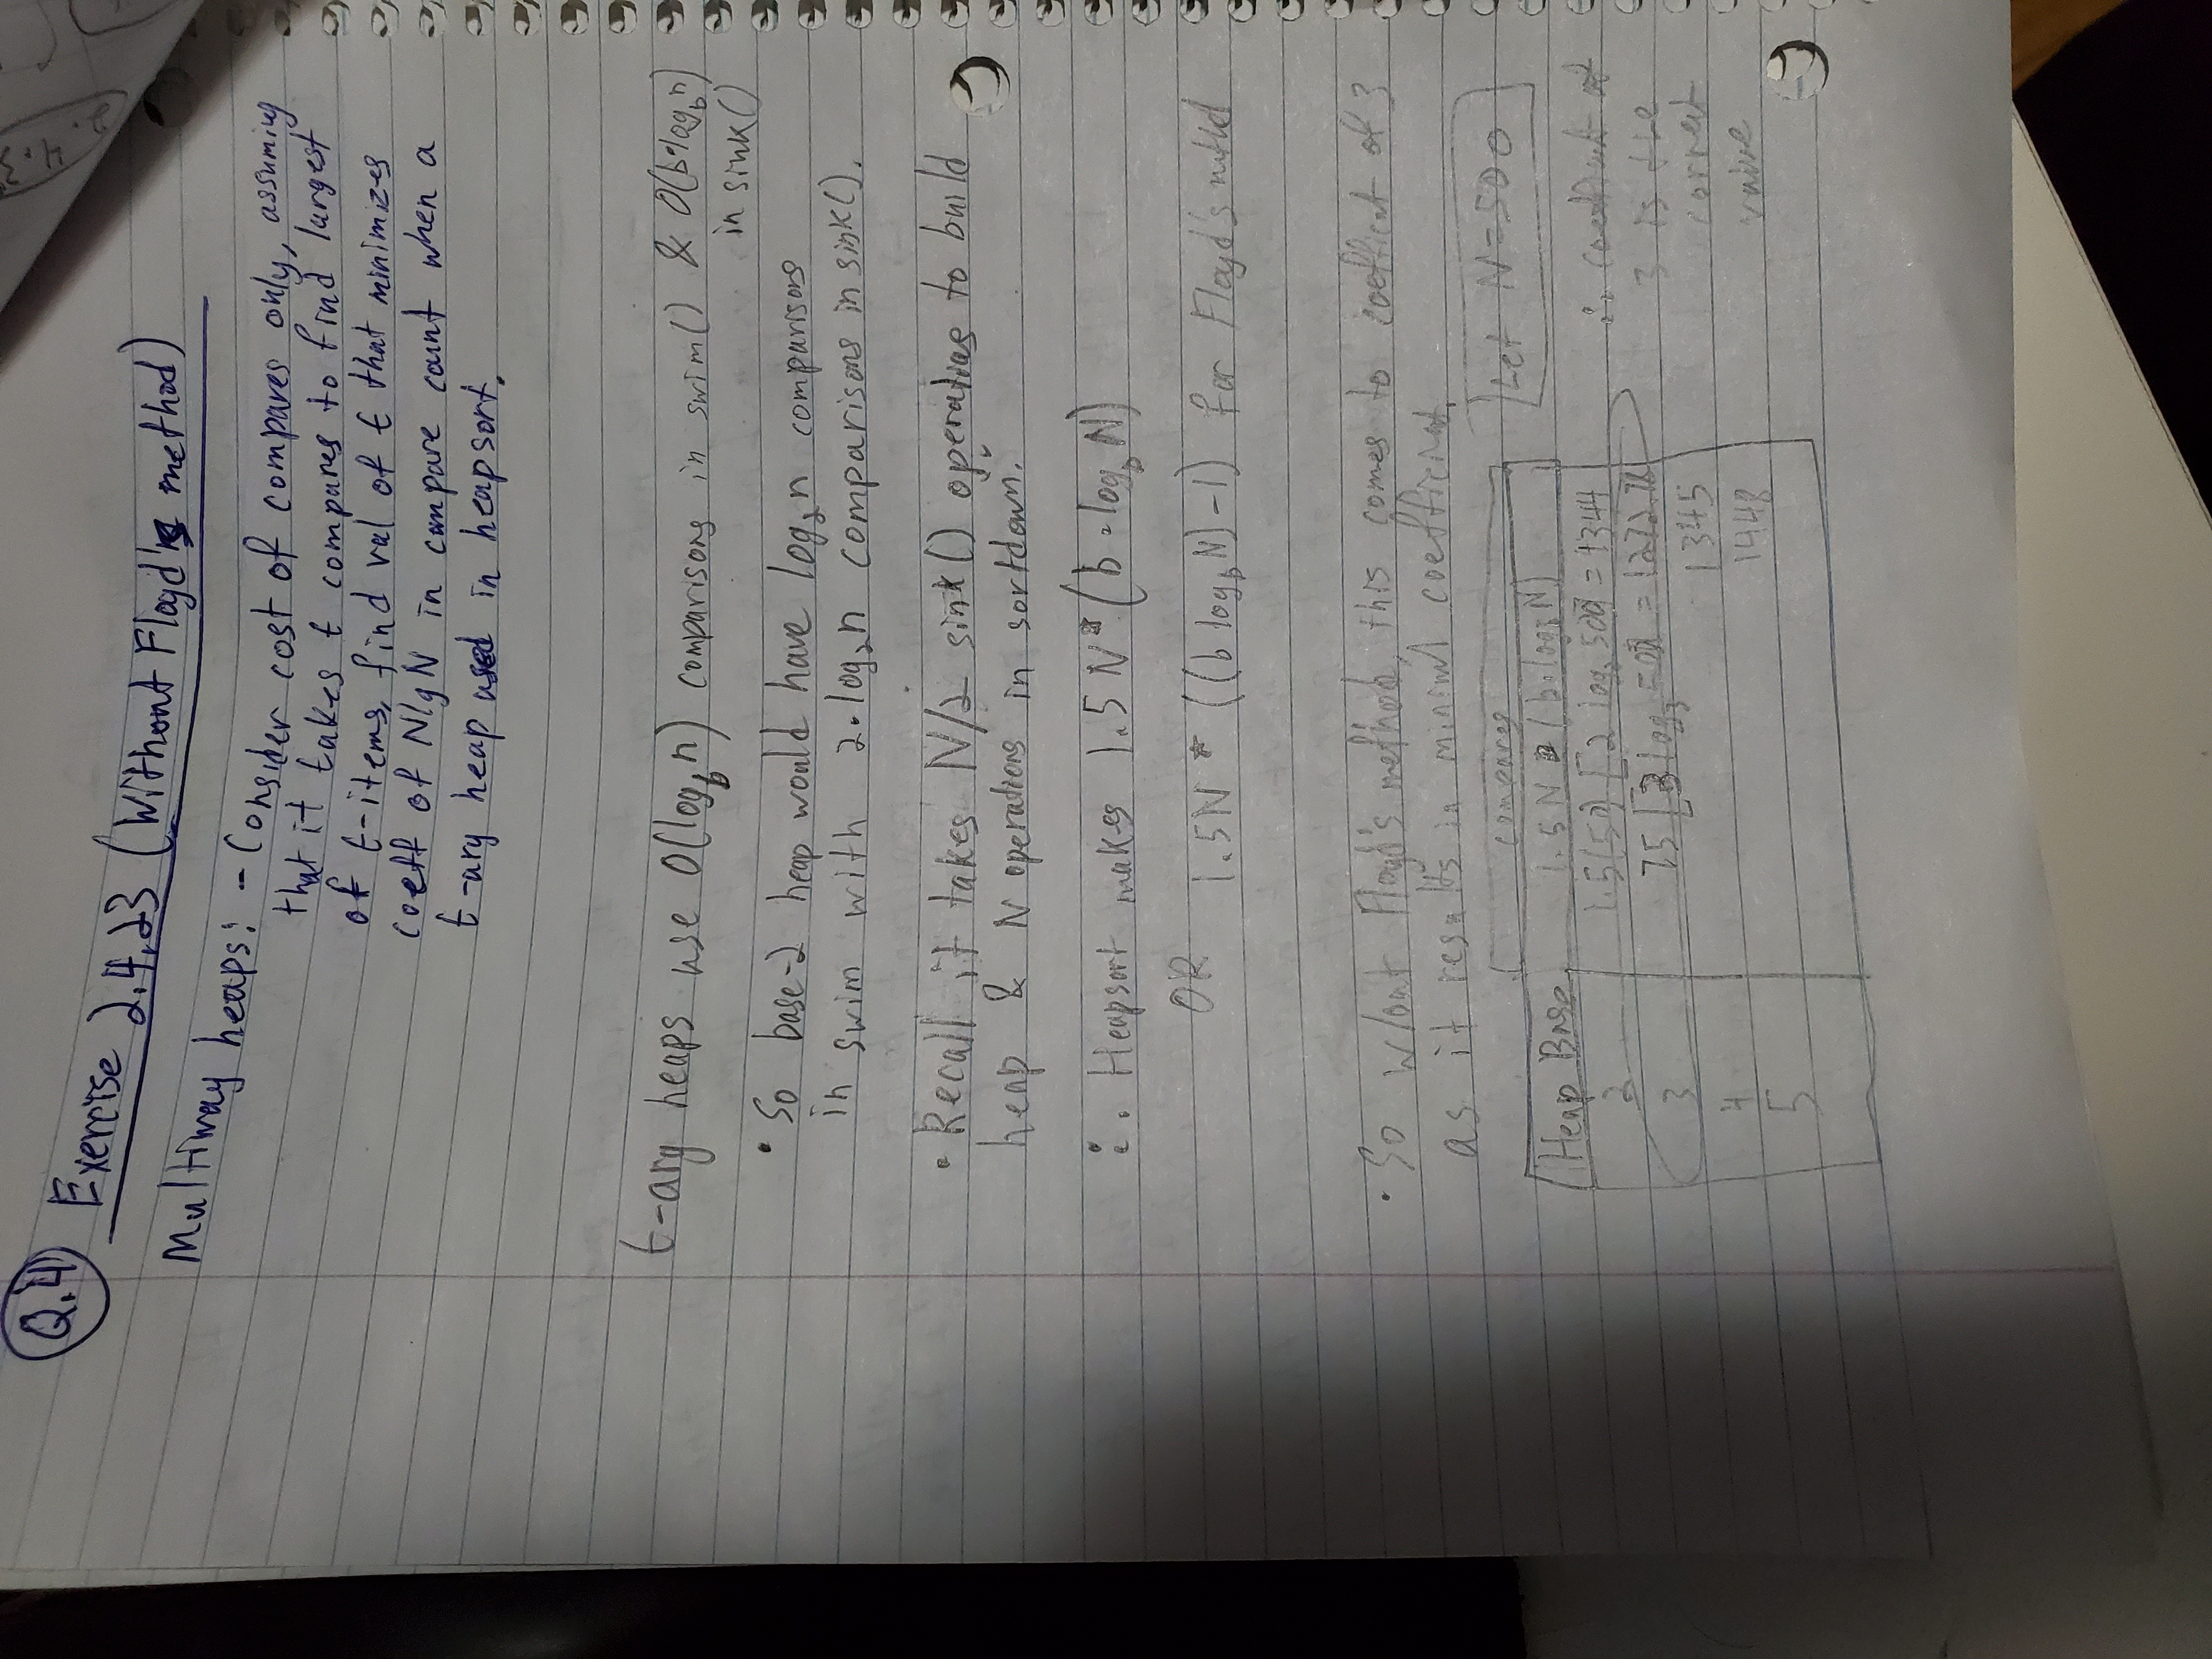
\includegraphics[scale=.1]{2.4.23.jpg}
\end{center}


\end{document}
